

\startappendix{State Space Model with Kalman Filter}
\label{chapter:appendixA}

%\input chapters/appendix/a1

We follow Koopman's (2002) notation and modify notation for convenience. 


\section{State Space Model}


Linear Gaussian state space model is defined in three parts:



\textbf{Observation/measurement equation}


The observations uncertainty $p(y_{t} \mid \mathbf{\alpha}_{t},\theta)$ described by the observation equation

$$y_{t} = F_{t}\alpha_{t}+v_{t},\quad  v_{t}\sim \mathcal NID(0,V_{t})$$



\textbf{State/transition/model equation} 


The process uncertainty of the unknown states $\alpha_{t}$ and their evolution given by the process equations as $p(\alpha_{t} \mid \theta)$.  


$$\alpha_{t} = G_{t}\alpha_{t-1}+B_{t} u_{t}+w_{t},\quad  w_{t}\sim \mathcal NID(0,W_{t})$$


\textbf{Parameters to estimated $p(\theta)$ }


$$\theta : { \alpha_t, F_t,  G_t ,V_{t}, W_{t} }$$


\textbf{The initial state distribution }



$$\alpha_{1}\sim \mathcal N(a_1,P_{1})$$




where 


-  $y_{t}$ is the observation of target variable  at time $t$ , with $t = 1,..., T$.



-  $\alpha_t$ is state vector (length $m$), the unobserved / hiden states of the system. In time series setting, $\alpha_t$ will have various components such as trend, seasonality, etc.  







-  $G_t$ is state transition model (A $m \times m$ matrix) which is applied to the previous state $\alpha_{t-1}$. The unobservaed state $x_t$ evolve in time according to the $G_t$. 







- $F_t$ is the observation model (a $m \times 1$)  matrix/vector which transforms the true state space into the observed space in our structral time series model. 







- $v_t$ is the measurement errors (observation noise) which is assumed to be zero mean Gaussian white noise with covariance $V_t$. In our structral time series model, it is a scalar/constant ;







- $w_t$ is the state innovations (the process noise) which is assumed to be drawn from a zero mean multivariate normal distribution with covariance $W_t$.







- $B_t$ is the model that predicts what changes based on  control/commands.







- $u_t$ is the control / commands/ input  in time $t$. In our model, we have not include any control or intervention policy, so no $B$ and $u$ terms are in our model. 




The initial state, and the noise vectors at each step ${\alpha_0, w_1, ..., w_t, v_1 ... v_t}$ are all assumed to be mutually \textit{independent}.





\section{Kalman Filter} 

Kalman Filter has two stages: 

\begin{enumerate}
	\item{Predicting the new state and its uncertainty}
	\item{Correcting with the new measurement}
\end{enumerate}





\subsection{The state of Kalman Filter}

The state of the filter is represented by two variables:conditional mean(expected value) and covariance.

$$p(\alpha_t \mid y_t) \sim N( \hat \alpha_{t \mid t}, P_{t \mid t})$$ 

\begin{enumerate}
	\item{$\hat{\alpha}_{t\mid t}$, the  posteriori state estimate at time $t$ given observations up to  and including at time $t$;}
	
	
	\item{$\mathbf{P}_{t\mid t}$, the posteriori error covariance matrix (a measure of the estimated accuracy of the state estimate). It reflects the variance of the state distribution.
		
		$$\mathbf{P}_{t\mid t} = \mathrm{cov}(\alpha_t - \hat{\alpha}_{t\mid t})$$
		
		$$\mathbf{P}_{t\mid t-1} = \mathrm{cov}(\alpha_t - \hat{\alpha}_{t\mid t-1})$$
		
		(? how do we know $\alpha_t$)
		}
	
\end{enumerate}




\subsection{Two phases: Predict and Correct} 


The Correct/measurement update adjusts the projected estimate by an actual measurement at that time.


\textbf{Predict/(state, error)stage/ (time update)} 


The Predict/time update projects the current state estimate ahead in time. 

$$\hat{\alpha}_{t\mid t-1} = \mathbf{G}_{t}\hat{\alpha}_{t-1\mid t-1} + \mathbf{B}_{t} \mathbf{u}_{t}$$



$$\mathbf{P}_{t\mid t-1} = \mathbf{G}_{t} \mathbf{P}_{t-1\mid t-1} \mathbf{G}_{t}^{\text{T}} + \mathbf{W}_{t}$$

where

$\hat{\alpha}_{t\mid t-1}$: Predicted (a priori) state estimate, which follows law of motion.  $G$ is not chosen by people, and it is the model of motion. $B$ and $u$ are control or intervention policy and can be chosen by people to change the state $\alpha$. $\hat{\alpha}_{t\mid t-1}$ is the estimate in next state; $\hat{\alpha}_{t-1\mid t-1}$ is the estimated state in last state. We know the initial state $\alpha_0$.    


$\mathbf{P}_{t\mid t-1}$: Predicted (a priori) estimate error covariance ahead. $\mathbf{P}_{t-1\mid t-1}$ the previous error covariance at time t-1.  

$\mathbf{W}$: the covariance of the error noise.








\textbf{Correct /Update stage/  measurement update}

The Correct/measurement update adjusts the projected estimate by an actual measurement at that time.


\textit{Updated (a posteriori) state estimate $\hat{\alpha}_{t\mid t}$} with new observation $y_t$. $\hat{\alpha}_{t\mid t}$ is a weighted average of latest estimate and gain from observation. 


$$\hat{\alpha}_{t\mid t} = \hat{\alpha}_{t\mid t-1} + \mathbf{K}_t \tilde{v}_t$$  


\textit{Updated (a posteriori) estimate covariance $\mathbf{P}_{t|t}$} 



$$\mathbf{P}_{t|t} = (I - \mathbf{K}_t \mathbf{F}_t) \mathbf{P}_{t|t-1}$$


$\mathbf{P}_{t|t}$ is new estimation error covariance. $\mathbf{P}_{t-1}$ is the previous estimate of the error noise. 


when the \textbf{prediction error}  $\tilde{v}_t$  is non-zero, there is new information about the system, so the state  $\alpha$ should be modified.


$\tilde{v}_t$ is also called Measurement innovation or the predictive residual.  

The prediction error $\tilde{v}_t$ reflects the discrepancy between the predicted measurement $E(y_{t\mid t-1})$ and the actual measurement $y_t$. In our case, the prediction error is a scalar $\tilde{v}_t$:

  
$$\begin{aligned}
\tilde v_t  &= y_t -E(y_{t\mid t-1} ) \\
& = y_t -E( F_{t}\alpha_{t}+v_{t\mid t-1} ) \\
& = y_t - F_{t} E(\alpha_{t\mid t-1} ) \\
& = y_t -F_{t} \hat \alpha_{t}
\end{aligned}$$

and the variance of $\tilde{v}_t$ is  

$$\mathbf{S}_{t} = \mathrm{cov}(\tilde{v}_t) 
 = \mathbf{F}_t \mathbf{P}_{t\mid t-1} \mathbf{F}_{t}^\text{T} + \mathbf{V}_t$$

where $V_t$ describes the noise in the observation $\mathbf{y}_t$.


The contribution of $\tilde{v}_t$ to the state vector is weighted by the \textbf{Optimal Kalman gain} $\mathbf{K}_t$. $\mathbf{K}_t$ measures how much to trust a new observation ${y}_t$. It can be matrix, and in our case it is a vector.



An \textbf{Optimal Kalman gain} $\mathbf{K}_t$ is chosen to be the gain or blending factor so that minimizes the a posteriori estimation error covariance equation $\mathbf{P}$.


$$\mathbf{K}_t = \mathbf{P}_{t\mid t-1}\mathbf{F}_t^T \mathbf{S}_t^{-1}$$



where $\mathbf{S}_t$ is prediction error covariance.  $\mathbf{F}_t$ describes  how the observation reflect the state in the model (a function of how much influence goes from observation to state vector).





The Kalman filter is a minimum mean-square error estimator. The error in the a posteriori state estimation is


$$\alpha_{t} - \hat{\alpha}_{t\mid t}$$

(But how do we know $\alpha_{t}$)


We seek to minimize the expected value of the square of the magnitude of this vector, $\textrm{E}[\|\alpha_{t} - \hat{\alpha}_{t|t}\|^2]$. This is equivalent to minimizing the trace of the a posteriori estimate covariance matrix $\mathbf{P}_{t|t}$ . Solving this optimization problem for $\mathbf{P}_{t|t}$ yields the optimal Kalman gain  $\mathbf{K}_t$:


$$\mathbf{K}_t \mathbf{S}_t = (\mathbf{H}_t \mathbf{P}_{t\mid t-1})^\text{T} = \mathbf{P}_{t\mid t-1} \mathbf{F}_k^\text{T}$$


$$\mathbf{K}_{t} = \mathbf{P}_{t\mid t-1} \mathbf{H}_t^\text{T} \mathbf{S}_t^{-1}$$


This gain  is  the optimal Kalman gain and yields MMSE estimates.  (P solves the associated Riccati equation. need citation)



The two phases alternate, with the prediction advancing the state until the next scheduled observation, and the update incorporating the observation. 


\startappendix{Data of Predictors}
\label{chapter:appendixB}

Predictors asre all seasonal adjusted, detrended, and scaled. They are all stationary and pass the ADF and KPSS test. 


\section{TSX stock market index}


TSX stock market index is daily and from 1980 to 2015/05/06

Before included in our model, it is transformed to log return and is detrended, deseasonalized and scaled to achieve stationary. 

In order to match up the quarterly target variable, it is skipping sampled as we mentioned at section 3.2.2. 

\begin{figure}[h]
\centering
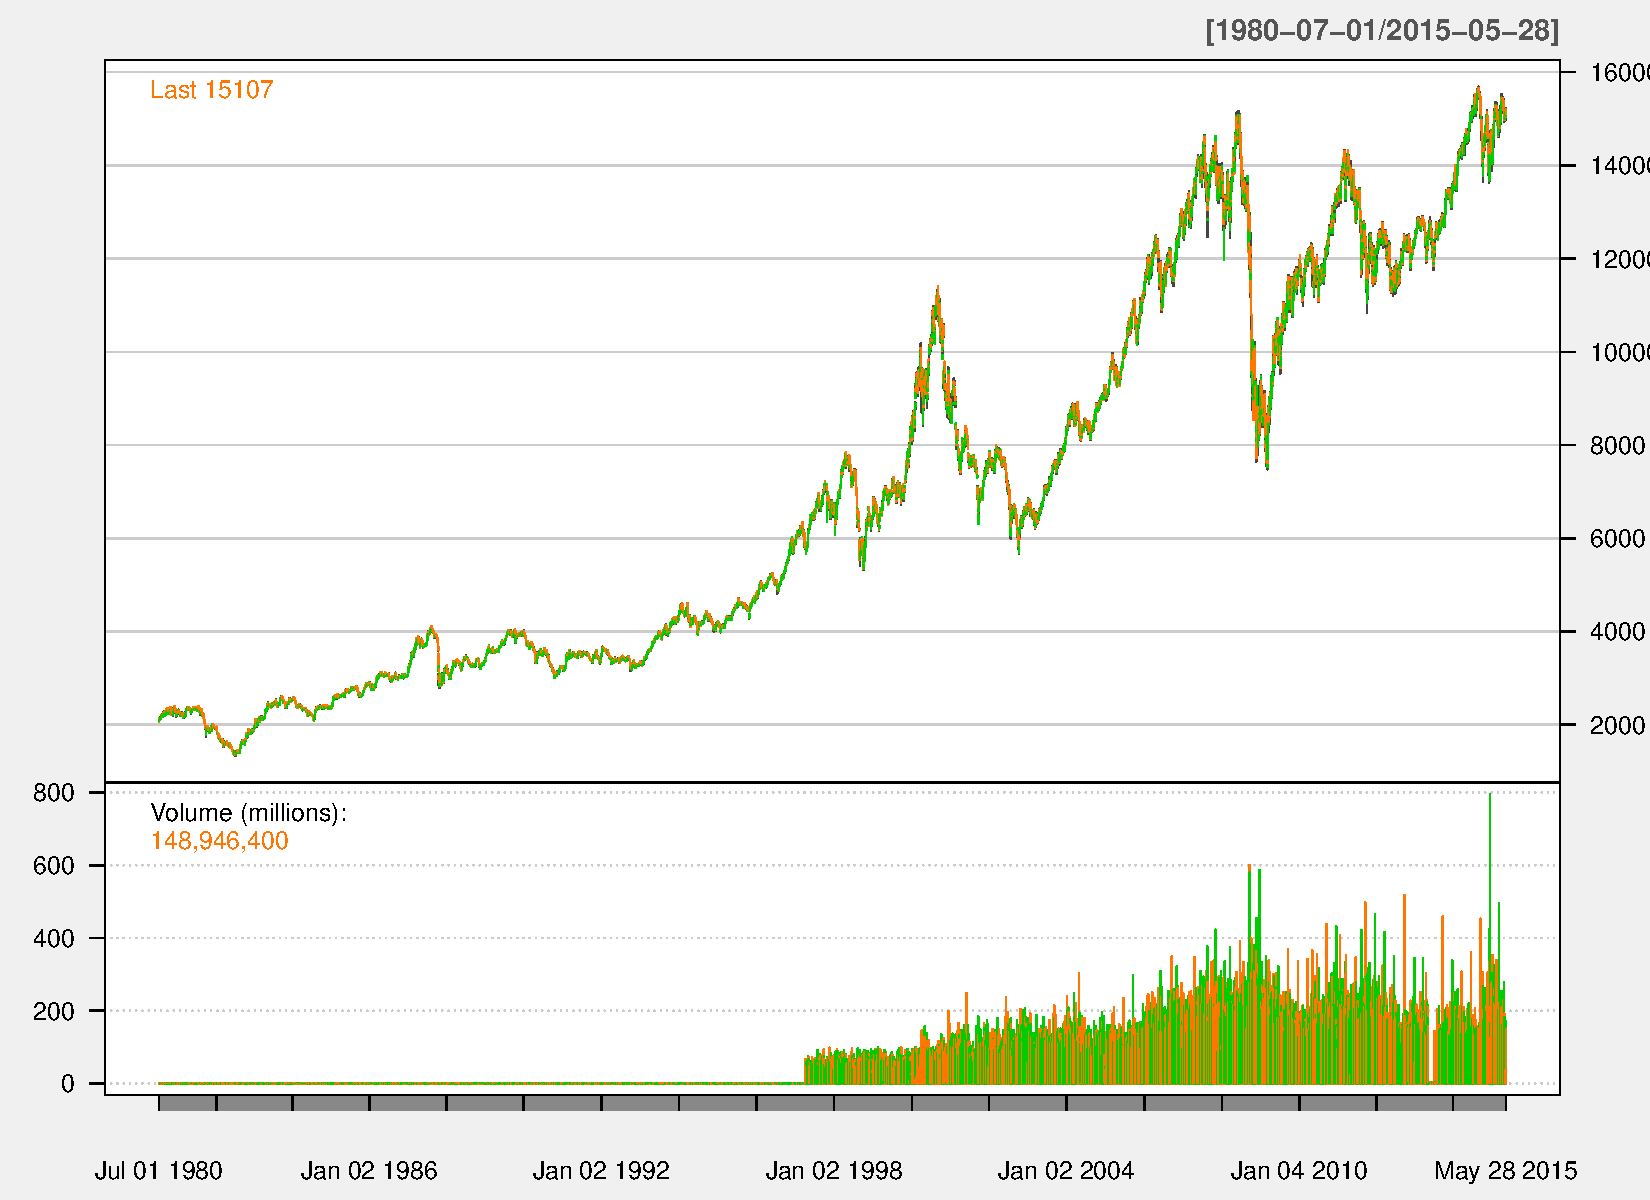
\includegraphics[width=0.7\linewidth]{Figures/tsx-report}
\caption{TSX stock market index}
\label{fig:tsx-report}
\end{figure}


\section{Unemployment rate: Monthly, 1956-2015/03}  


Unemployment Rate: Aged 15 and Over: All Persons for Canada

2015-03: 6.6 Percent

Monthly, Seasonally Adjusted, Updated: 2015-05-06

Unemployment rate is detrended, deseasonalized and scaled. And then it is skipping sampled as we mentioned at section 3.2.2. 

\begin{figure}[h]
\centering
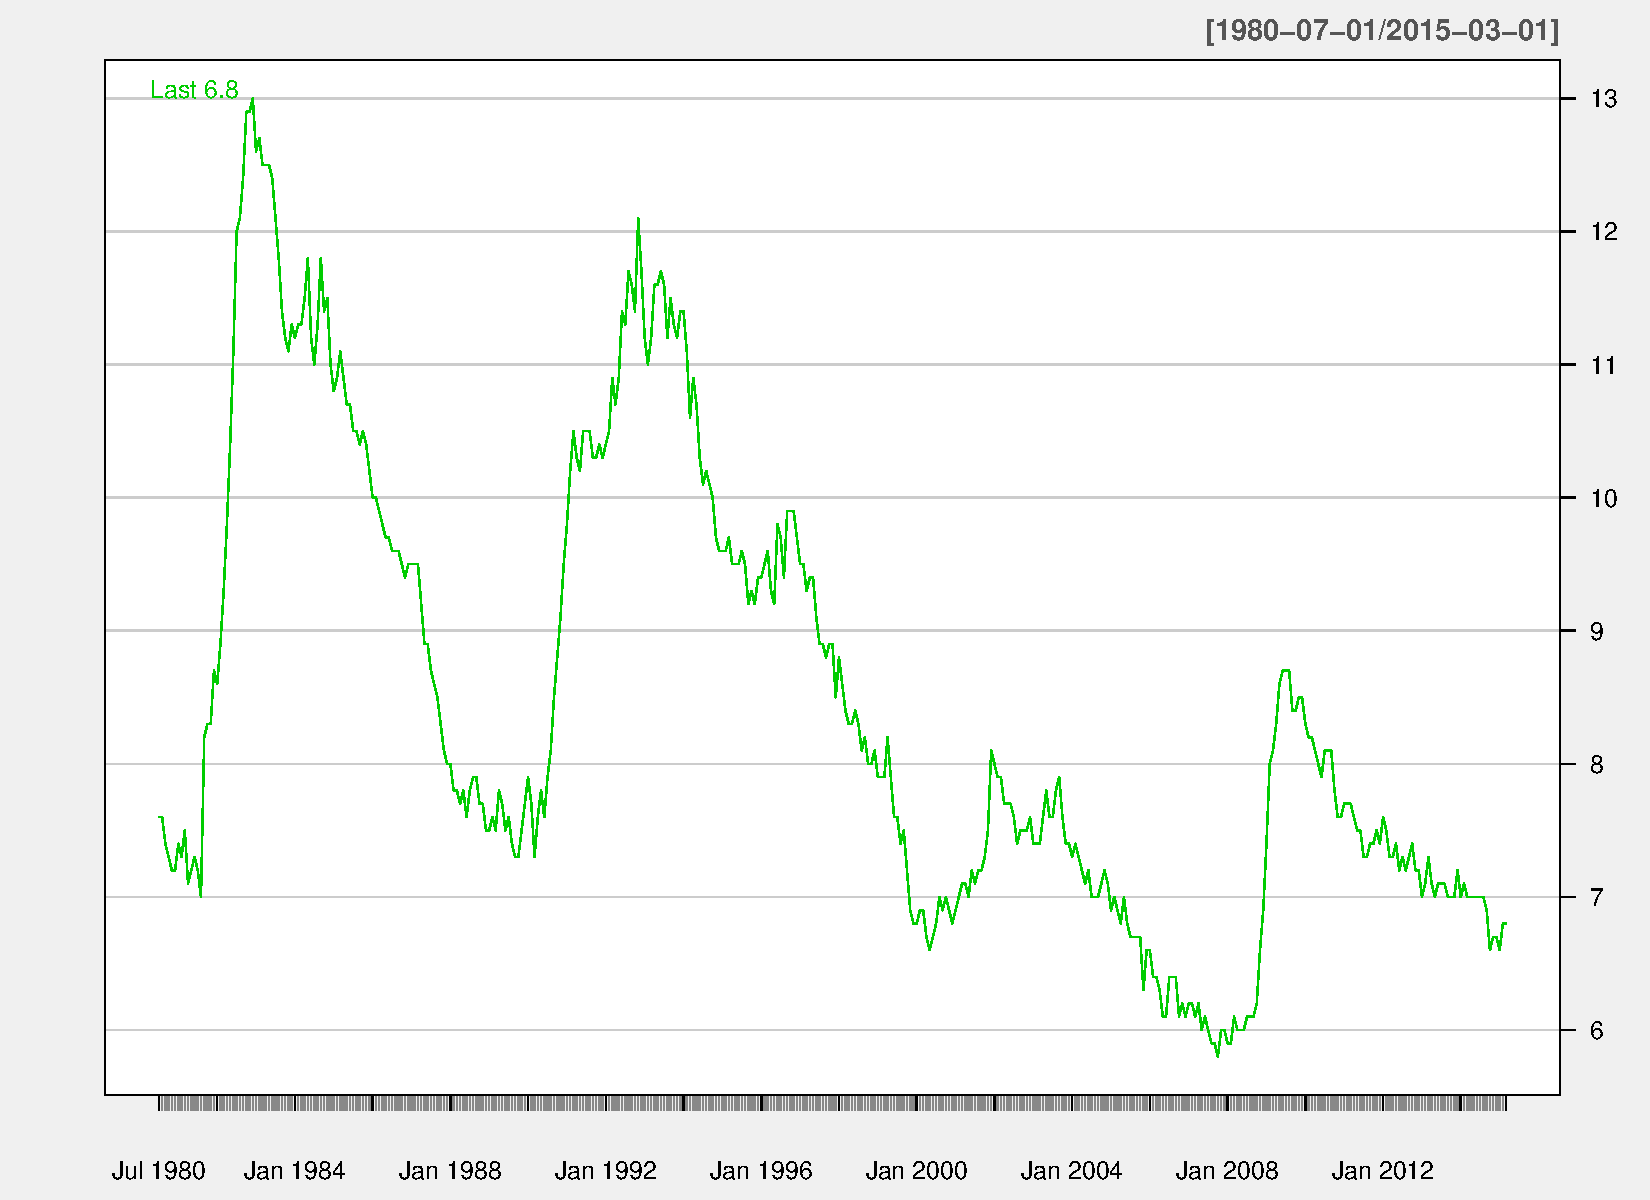
\includegraphics[width=0.7\linewidth]{Figures/labor-report}
\caption{Unemployment Rate}
\label{fig:labor-report}
\end{figure}
 
 
\section{Spread between 3 month and 10 year government bond interest rate. Monthly, 1956 - 2015/02} 
 
 
\begin{enumerate}
	\item{Long-Term Government Bond Yields: 10-year: Main (Including Benchmark) for Canada
		
		2015-02: 1.38000 Percent
		
		Monthly, Not Seasonally Adjusted, Updated: 2015-05-06}
	\item{3-Month or 90-day Rates and Yields: Interbank Rates for Canada
		
		2015-02: 0.89000 Percent 
		
		Monthly, Not Seasonally Adjusted, Updated: 2015-05-06}
\end{enumerate} 
 




The spread is the difference between the 3 month's interest rate and 10 year's government bond interest rate. 

 
It is detrended, deseasonalized and scaled. And then it is skipping sampled as we mentioned at section 3.2.2. 
 
 
\begin{figure}
\centering
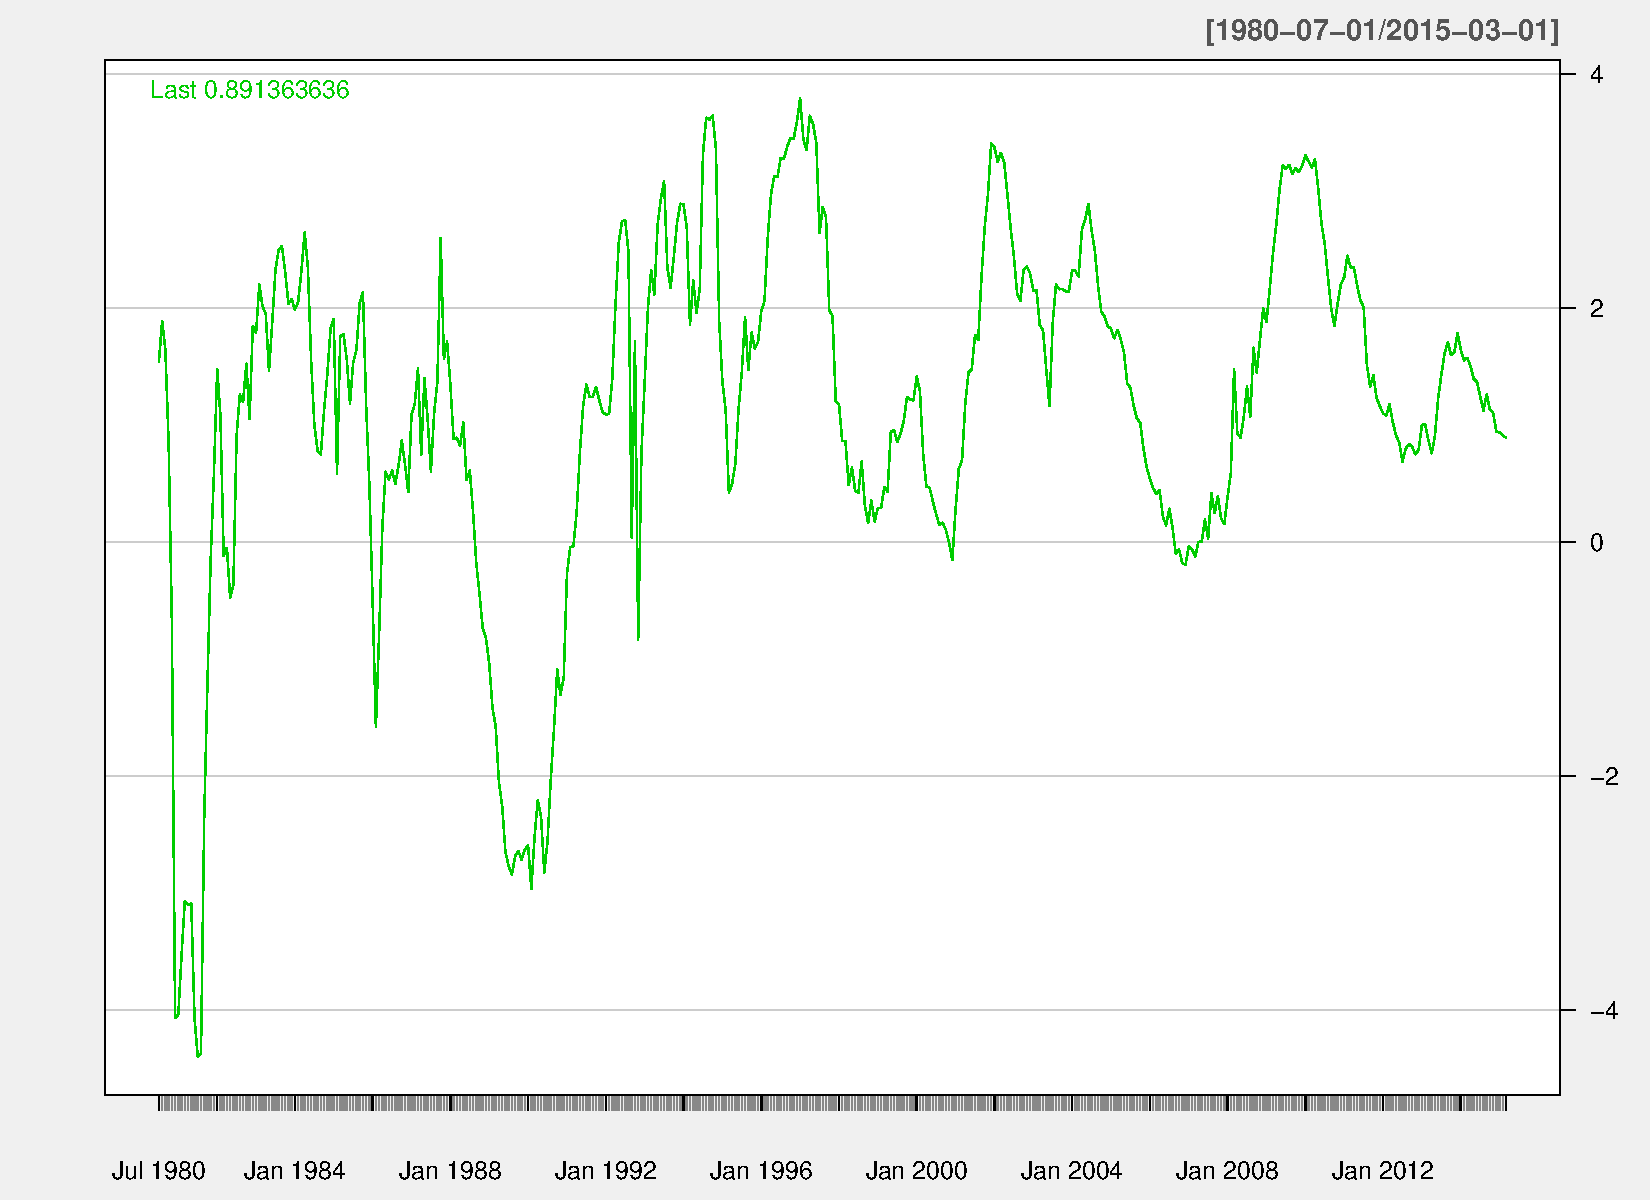
\includegraphics[width=0.7\linewidth]{Figures/spread-report}
\caption{Spread between 3 month and 10 year government bond interest rate}
\label{fig:spread-report}
\end{figure}


\section{Housing starts, monthly, 1948-2015/02} 

Canada Mortgage and Housing Corporation, housing starts, under construction and completions in centres 10,000 and over, Canada, provinces, selected census metropolitan areas

monthly (units) Updated: 2015-05-06 

It is detrended, deseasonalized and scaled. And then it is skipping sampled as we mentioned at section 3.2.2. 

\begin{figure}
\centering
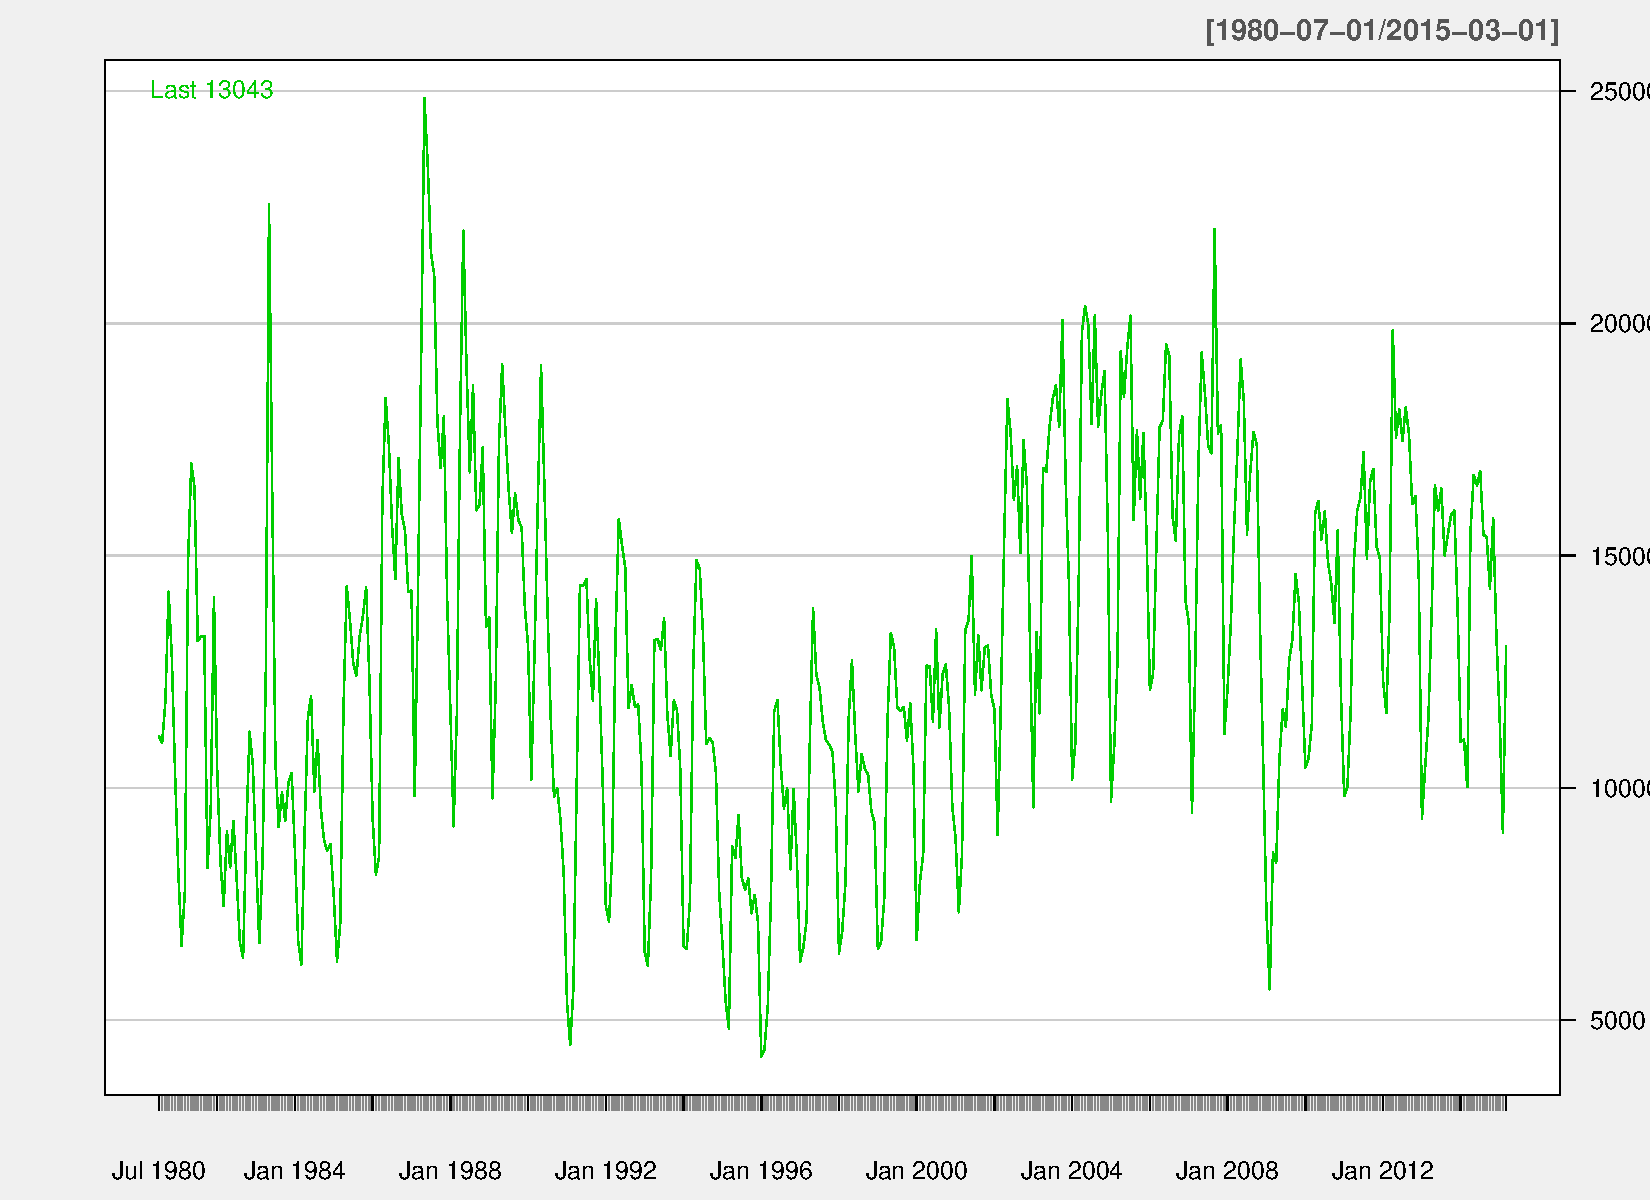
\includegraphics[width=0.7\linewidth]{Figures/house-report}
\caption{Housing starts}
\label{fig:house-report}
\end{figure}





\startappendix{Model Specification}
\label{chapter:appendixC}

\section{AR(1) Model}

$$y_t = \beta_0 + a_1 y_{t-1} +v_{t}, \quad v_{t} \sim N(0, V)$$



AR(1) model is selected by `auto.arima` function in `forecast` package in R. The parameters are estimated by the `arima` function. The forecasting is estimated by `fitted` function. 



\section{Generalized local trend model with regression}


The generalized local linear trend model is more complicated than regular local trend model. 



\textbf{Observation equation} (level + regression): 



$$y_t = \mu_t + z_t + v_{t}, \quad v_{t} \sim N(0, V)$$



It assumes the level moves according to a random walk, but the slope moves according to an AR1 process centered on some potentially nonzero value D. The equation for the mean is


\textbf{State equation 1} (random walk + trend ):  



$$\mu_{t+1} = \mu_{t} + b_{t} +  w_{1t}, \quad w_{1t} \sim N(0, W_{1})$$



The equation for the slope $b$  is



\textbf{State equation} 2 ( AR(1) for trend):  



$$b_{t+1} = D + \phi * (b_t - D) + w_{2t}, \quad w_{2t} \sim N(0, W_{2})$$



The prior distribution for this model has four independent components. There is an inverse gamma prior on the level standard deviation sigma.level, an inverse gamma prior on the slope standard deviation sigma.slope, a Gaussian prior on the long run slope parameter $D$, and a potentially truncated Gaussian prior on the AR1 coefficient $\phi$. If the prior on $\phi$ is truncated to (-1, 1), then the slope will exhibit short term stationary variation around the long run slope $D$ (Scott, 2014, R document).




\textbf{State equation} 3 (regression): $$z_t = \beta x_t$$




\section{Reference}



Altissimo, F., Cristadoro, R., Forni, M., Lippi, M., and Veronese, G. (2010). New Eurocoin: Tracking Economic Growth in Real Time. The Review of Economics and Statistics, 92(4), 1024–1034. Retrieved from http://ideas.repec.org/a/tpr/restat/v92y2010i4p1024-1034.html



An, O. (2011). Forecasting Commodity Prices with Mixed Frequency Data: An OLS Based Generalized ADL Approach. Retrieved from http://www.econ.sinica.edu.tw/upload/file/(20111020)(1).pdf



Andreou, E., Ghysels, E., and Kourtellos, A. (2013). Should Macroeconomic Forecasters Use Daily Financial Data and How? Journal of Business and Economic Statistics, 31(2), 240-251. doi:10.1080/07350015.2013.767199


Avi Goldfarb, Shane Greenstein, and Catherine Tucker. (2015). Economic Analysis of the Digital Economy. Book, University of Chicago Press. Retrieved from http://www.nber.org/books/gree13-1

Bai, J., Ghysels, E., and Wright, J. H. (2013). State Space Models and MIDAS Regressions. Econometric Reviews, 32(7), 779–813. doi:10.1080/07474938.2012.690675



Bai, J., and S. Ng (2009), Boosting Diffusion Indexes,Journal of Applied Econometrics, 24, 607-629.



Bai, J., and S. Ng (2008), Large Dimensional Factor Models, Foundations and Trends in Econometrics, 3, 89-163



Bańbura, M., Giannone, D., Modugno, M., and Reichlin, L. (2013). Wo r k i n g Pa p e r S e r i e S the real-time data flow NOTE : This Working Paper should not be reported as representing, (15).


Bencivelli, Lorenzo and Marcellino, Massimiliano Giuseppe and Moretti, Gianluca, Selecting Predictors by Using Bayesian Model Averaging in Bridge Models (July 26, 2012). Bank of Italy Temi di Discussione (Working Paper) No. 872. Available at SSRN: http://ssrn.com/abstract=2154928 or http://dx.doi.org/10.2139/ssrn.2154928 


Bencivelli, L., Marcellino, M., and Moretti, G. (2012). Selecting predictors by using Bayesian model averaging in bridge models. Temi Di Discussione (Economic Working Papers). Retrieved from http://ideas.repec.org/p/bdi/wptemi/td\_872\_12.html

Bencivelli, Lorenzo and Marcellino, Massimiliano Giuseppe and Moretti, Gianluca, Selecting Predictors by Using Bayesian Model Averaging in Bridge Models (July 26, 2012). Bank of Italy Temi di Discussione (Working Paper) No. 872. Available at SSRN: http://ssrn.com/abstract=2154928 or http://dx.doi.org/10.2139/ssrn.2154928 


Boriss Siliverstovs (2015). Short-term forecasting with mixed-frequency data: A MIDASSO approach. Retrieved from http://www.kof.ethz.ch/en/publications/p/kof-working-papers/158/

Brodersen, B. K. H., Gallusser, F., Koehler, J., Remy, N., and Scott, S. L. (2014). Inferring causal impact using Bayesian structural time-series models. Annals of Applied Statistics.

Buchen, T., and Wohlrabe, K. (2011). Forecasting with many predictors: Is boosting a viable alternative? Economics Letters, 113(1), 16-18. doi:10.1016/j.econlet.2011.05.040








Carriero, A., Clark, T. E., and Marcellino, M. (2015). Realtime nowcasting with a Bayesian mixed frequency model with stochastic volatility. Journal of the Royal Statistical Society: Series A (Statistics in Society).  http://doi.org/10.1111/rssa.12092



Castle, J., and Hendry, D. (2013). Forecasting and Nowcasting Macroeconomic Variables: A Methodological Overview. Economics Series Working Papers. Retrieved from http://ideas.repec.org/p/oxf/wpaper/674.html


Clements, M. P., and Galvão, A. B. (2008). Macroeconomic Forecasting With Mixed-Frequency Data: Forecasting Output Growth in the United States, (May 2015), 37-??41. doi:10.1198/073500108000000015







De Mol, C., Giannone, D., and Reichlin, L. (2008). Forecasting using a large number of predictors: Is Bayesian shrinkage a valid alternative to principal components? Journal of Econometrics, 146(2), 318-328. doi:10.1016/j.jeconom.2008.08.011   





Ferrara, L., and Marsilli, C. (2013). Variable selection with mixed frequencies : an assessment based on macroeconomic forecasting.





Foroni, C., M. Marcellino, and C. Schumacher, 2011. U-MIDAS: MIDAS regressions with unrestricted lag polynomials. Discussion Paper Series 1: Economic Studies No. 35/2011, Deutsche Bundesbank.





Foroni, C., and Marcellino, M. (2013). A Survey of Econometric Methods for Mixed-Frequency Data. doi:10.2139/ssrn.2268912

Frale, C., Marcellino, M., Mazzi, G. L., and Proietti, T. (2011). EUROMIND: a monthly indicator of the euro area economic conditions. Journal of the Royal Statistical Society: Series A (Statistics in Society), 174(2), 439–470. doi:10.1111/j.1467-985X.2010.00675.x

Ghysels, E., P. Santa-Clara, and R. Valkanov, 2006. Predicting volatility: Getting the most out of return data sampled at different frequencies. Journal of Econometrics, 131, 59-95.



Harvey, A. (2006). Chapter 7 Forecasting with Unobserved Components Time Series Models. Handbook of Economic Forecasting. doi:10.1016/S1574-0706(05)01007-4



Harvey, a C., and Peters, S. (1990). Estimation Procedures for Structural Time Series Models. Journal of Forecasting, 9(June 1988), 89-??108.



Hendry, D. F., and Hubrich, K. (n.d.). Combining disaggregate forecasts or combining disaggregate information to forecast an aggregate. Working Paper Series. Retrieved from http://ideas.repec.org/p/ecb/ecbwps/20101155.html



Hendry, D., and Mizon, G. E. (2012). Forecasting from Structural Econometric Models. Economics Series Working Papers. Retrieved from http://ideas.repec.org/p/oxf/wpaper/597.html











Koop, G., and Potter, S. (2004) find Bayesian model averaging in a dynamic factor model outperforms a single model for the problem of macroeconomic forecasting. 



Koop, G., and Korobilis, D. (2010). Forecasting In inflation using dynamic model averaging. International Economic Review, 53(3), 867-886.







Koop, G., and Potter, S. (2004). Forecasting in dynamic factor models using Bayesian model averaging. The Econometrics Journal, 7, 550-565. Retrieved from http://onlinelibrary.wiley.com/doi/10.1111/j.1368-423X.2004.00143.x/full



Marcellino and Schumacher (2010), we analyze the approach that merges factor models and the MIDAS f






Ng, S., and Wright, J. H. (2013). Facts and Challenges from the Great Recession for Forecasting and Macroeconomic Modeling. Journal of Economic Literature, 51(4), 1120-1154. doi:10.1257/jel.51.4.1120





Ouysse, R. (2013). Forecasting using a large number of predictors: Bayesian model averaging versus principal components regression.






Scott, S. L., and Varian, H. R. (2014). Bayesian Variable Selection for Nowcasting Economic Time Series. Economics of Digitization, (July 2014), 1–22. Retrieved from http://www.nber.org/papers/w19567.pdf


Stock, J., and Watson, M. (2006). Dynamic factor models. Oxford Handbook of Economic Forecasting, (January), 1-43. Retrieved from http://link.springer.com/article/10.1007/s10182-006-0219-z







Stock, J., and Watson, M. (2012). Generalized shrinkage methods for forecasting using many predictors. Journal of Business and Economic Statistics, 30(4), 481-493. doi:10.1080/07350015.2012.715956  














Wohlrabe, K., and Buchen, T. (2014). Assessing the Macroeconomic Forecasting Performance of Boosting: Evidence for the United States, the Euro Area and Germany. Journal of Forecasting, 33(4), 231-242. Retrieved from http://ideas.repec.org/a/wly/jforec/v33y2014i4p231-242.html
